%-*- Mode:LaTeX; -*-      
\documentclass[11pt]{article}
\usepackage{vmargin}		% Force narrower margins
\setpapersize{USletter}
\setmarginsrb{1.0in}{1.0in}{1.0in}{0.6in}{0pt}{0pt}{0pt}{0.4in}
\setlength{\parskip}{.1in}  % removed space between paragraphs
\setlength{\parindent}{0in}

\usepackage{epsfig}
\usepackage{graphicx}

\newcommand{\ra}{$\rightarrow$~}
\newcommand{\dt}{$\circ$~}

\begin{document}

\large
\begin{center}
{\bf CS-5340/6340, Written Assignment \#2} \\
Marek Baranowski
\end{center}
\normalsize

\begin{enumerate}  

\item (28 pts) Assume that a part-of-speech tagger has been applied to the
sentence below with the following results:

\begin{quote}
the/{\sc art~}  light/{\sc adj~}  green/{\sc adj~} 
  candle/{\sc noun~}  shines/{\sc verb~}  green/{\sc adj~}
 light/{\sc noun~} \\  in/{\sc prep~}  the/{\sc art~} 
  green/{\sc adj~}  room/{\sc noun~}  to/{\sc inf~} 
  light/{\sc verb~}  the/{\sc art~}  room/{\sc noun~}
\end{quote}
\vspace*{.2in}

Fill in the table below with the probabilities that you would estimate
based on the sentence above. \underline{Leave your results in fractional
  form! For example: 5/5}

\vspace*{.1in}
We define unigram, bigram , trigram, and emission probabilities as:
\begin{description}
\item[Lexical Unigram:] $P(w_i)$ means probability of word $w_i$
\item[POS Unigram:] $P(t_i)$ means probability of POS tag $t_i$
\item[Lexical Bigram:] $P(w_i \mid w_{i-1})$ means probability of word
  $w_i$ following word $w_{i-1}$
\item[POS Bigram:] $P(t_i \mid t_{i-1})$ means probability of POS
  tag $t_i$ following POS tag $t_{i-1}$
\item[Lexical Trigram:] $P(w_i \mid w_{i-2}~w_{i-1})$ means probability of word
  $w_i$ following words $w_{i-2}$ $w_{i-1}$
\item[POS Trigram:] $P(t_i \mid t_{i-2}~t_{i-1})$ means probability of word
  $t_i$ following words $t_{i-2}$ $t_{i-1}$
\item[Emission Probability:] $P(w_i \mid t_i)$ means
  probability of word $w_i$ given tag $t_i$.
\end{description}


 \begin{center}
 \begin{tabular}{|l|l|} \hline
 \textbf{Probability~~~~~~~~~~~~~~~} & \textbf{Value~~~~~~~~~~~~~~~~~} \\ \hline
 $P$(the) & 3/15 \\
 $P$(room) & 2/15 \\
 $P$(ADJ) & 4/15 \\
 $P$(VERB) & 2/15 \\
 $P$(room $\mid$ the) & 1/3 \\
 $P$(the $\mid$ in) & 1/1 \\
 $P$(candle $\mid$ light) & 0/3 \\
 $P$(in $\mid$ green light) & 1/1 \\
 $P$(NOUN $\mid$ ART) & 1/3 \\
 $P$(ADJ $\mid$ ADJ) & 1/4 \\
 $P$(PREP $\mid$ NOUN VERB) & 0/1 \\
 $P$(NOUN $\mid$ ART ADJ) & 1/2 \\
 $P$(the $\mid$ ART) & 3/3 \\
 $P$(green $\mid$ ADJ) & 3/4 \\ \hline
 \end{tabular}
 \end{center}
 

\newpage

\item (28 pts) Consider the following grammar G: 

\begin{center}
\begin{tabular}{|ll|} \hline
S \ra NP VP &      NP \ra John \\
S \ra NP VERB   &  NOUN \ra John \\   
NP \ra NOUN NP &  NP \ra Mary \\
VP \ra VERB NP &  NOUN \ra Mary \\
VP \ra VERB DITRANS & NP \ra fish \\
DITRANS \ra NP NP & NOUN \ra fish \\
VERB \ra bought & VERB \ra fish \\ \hline
\end{tabular}
\end{center}

\begin{enumerate}

\item Show the entries of the chart that would be produced by the
CKY parsing algorithm when parsing is completed for the sentence
{\bf ``John bought Mary fish''}.  Each entry [i,j] refers to the cell of the
chart for row i and column j. For example, chart[1,4]
refers to entries that span words 1 through 4.  \\

\noindent {\bf chart[1,1] : \{NP, NOUN\}} \\
\noindent {\bf chart[1,2] : \{S\}} \\
\noindent {\bf chart[1,3] : \{S\}} \\
\noindent {\bf chart[1,4] : \{S, S\}} \\
\noindent {\bf chart[2,2] : \{VERB\}} \\
\noindent {\bf chart[2,3] : \{VP\}} \\
\noindent {\bf chart[2,4] : \{VP, VP\}} \\
\noindent {\bf chart[3,3] : \{NP, NOUN\}} \\
\noindent {\bf chart[3,4] : \{DITRANS, S, NP\}} \\
\noindent {\bf chart[4,4] : \{NP, NOUN, VERB\}} \\

\item For \underline{every} S constituent in the chart, draw the parse
  tree for the structure that it represents. For each one,
  please indicate which cell the S constituent appeared in.
  
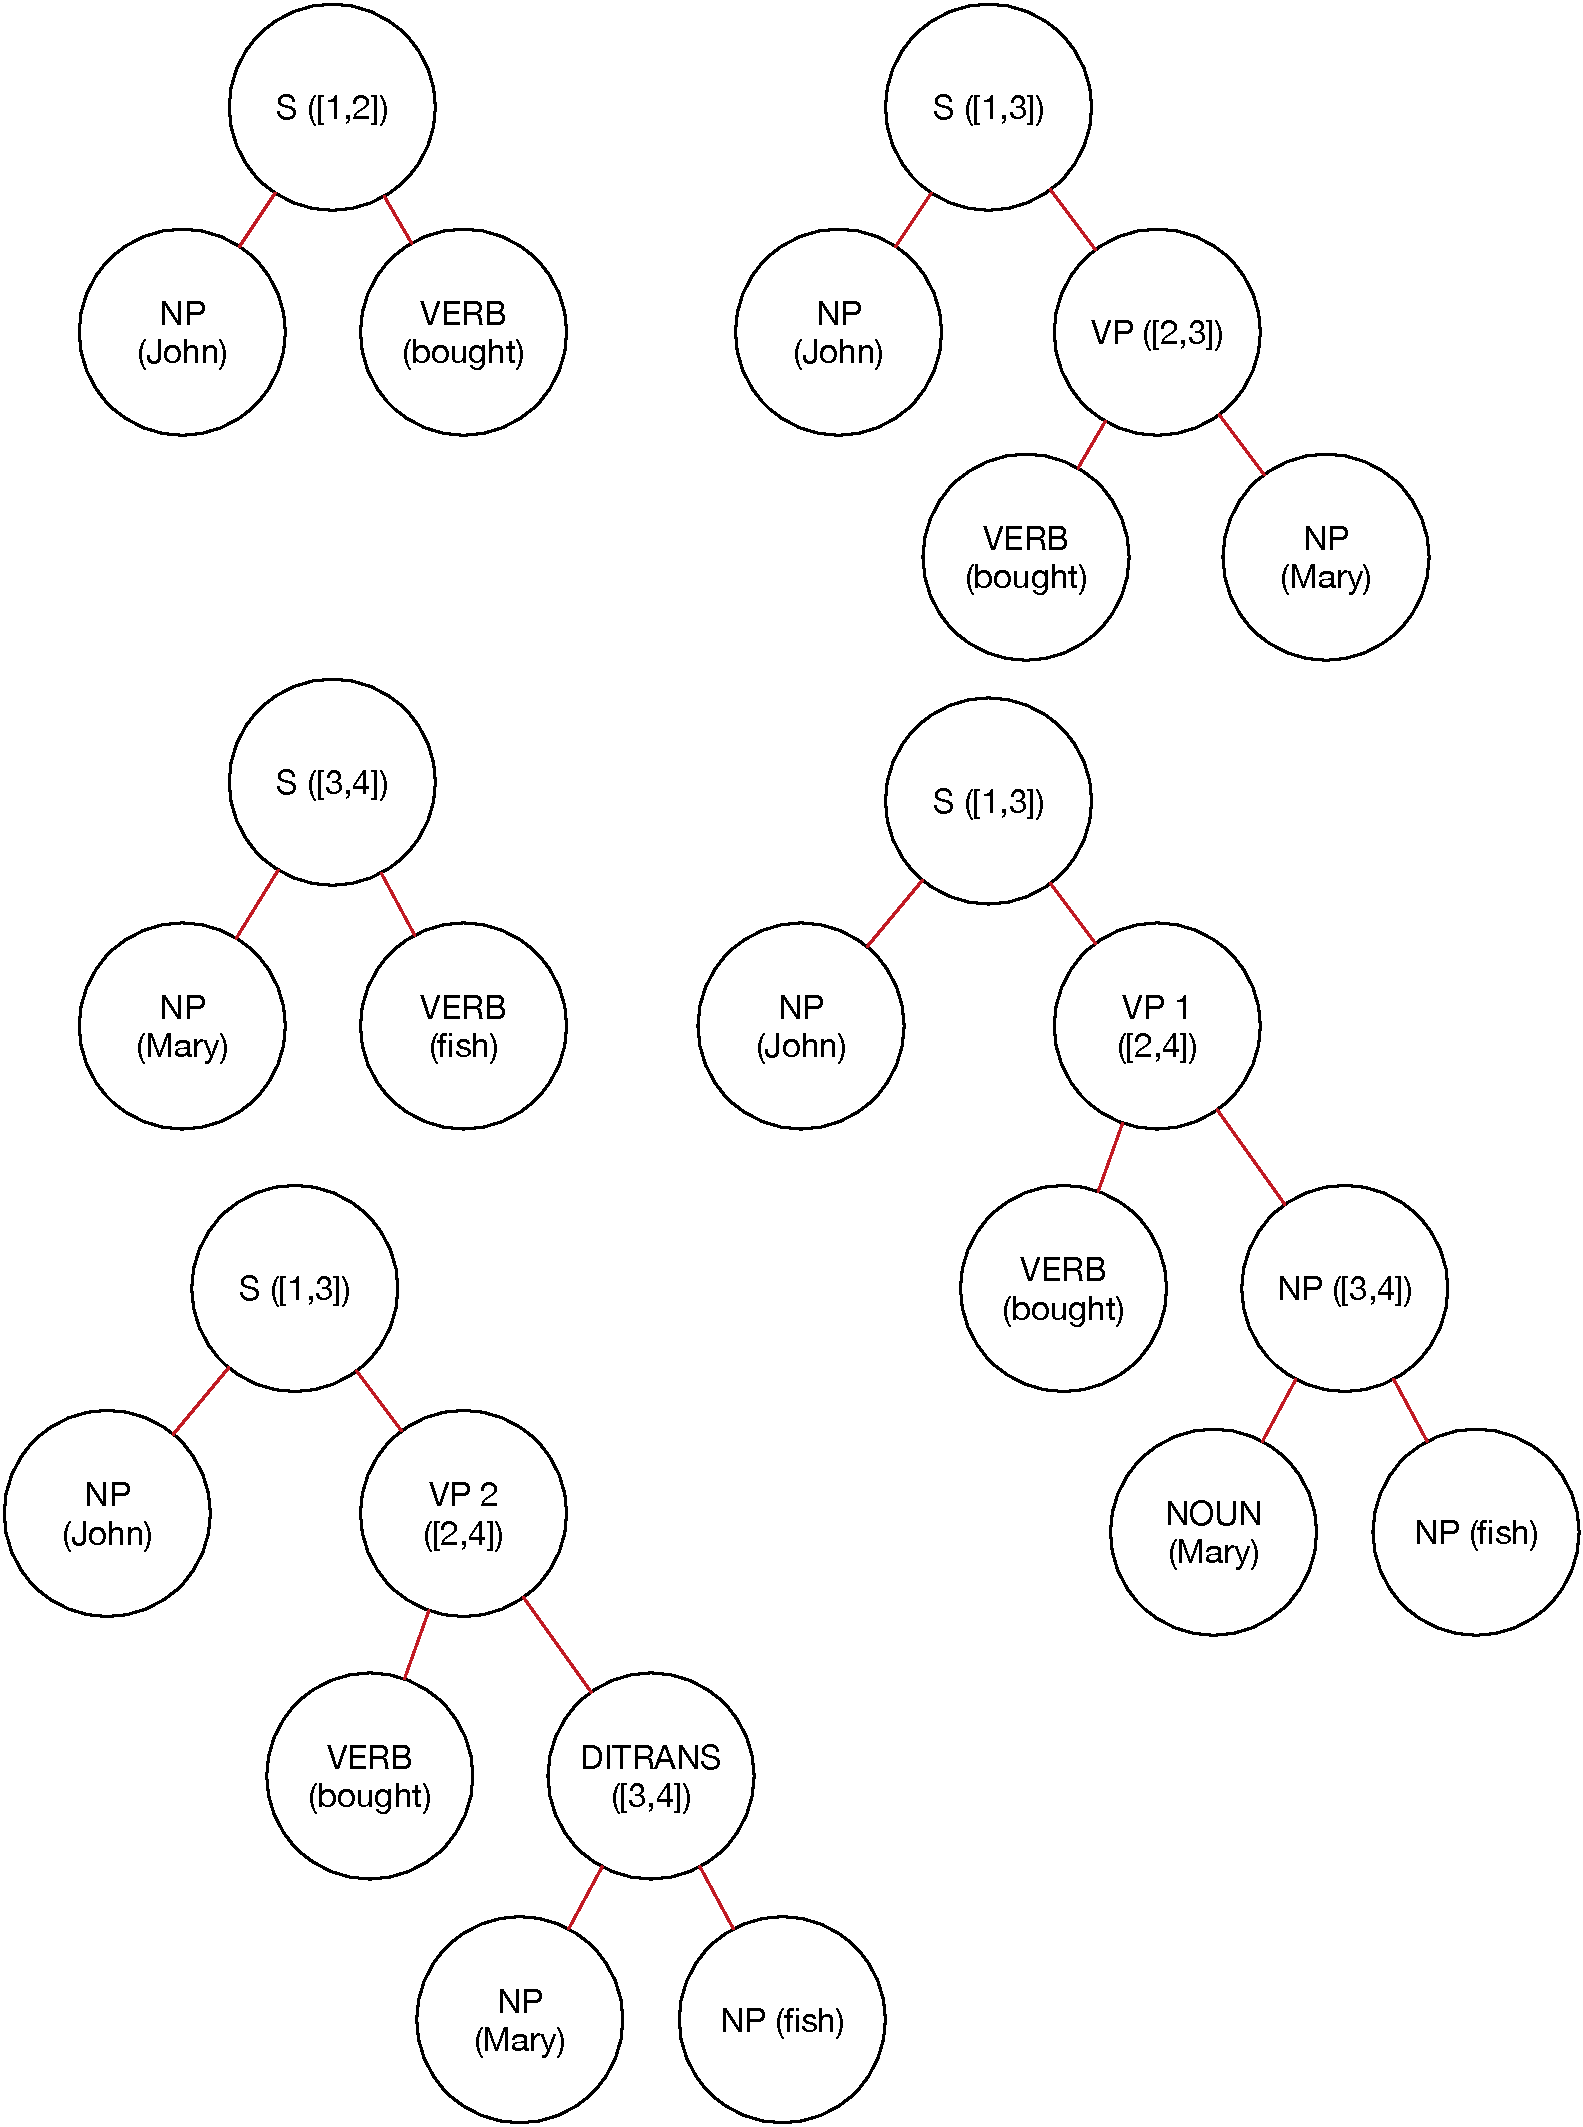
\includegraphics[width=0.5\textwidth]{Parses.pdf}

\end{enumerate}


\newpage
\item (15 pts) For each grammar below, draw a finite-state machine (FSM) that accepts
  exactly the same sequence of part-of-speech tags as the FSM.

\begin{enumerate}

\item Grammar \#1: \\ ~ \\
VP \ra adv VP \\
VP \ra verb VP1 \\
VP1 \ra adv VP1 \\
VP1 \ra adv \\
FSMs are presented in unsimplified form according to the algorithm from Sipser for right-linear grammars. The $\lambda$ symbol indicates a transition on the empty string.\\
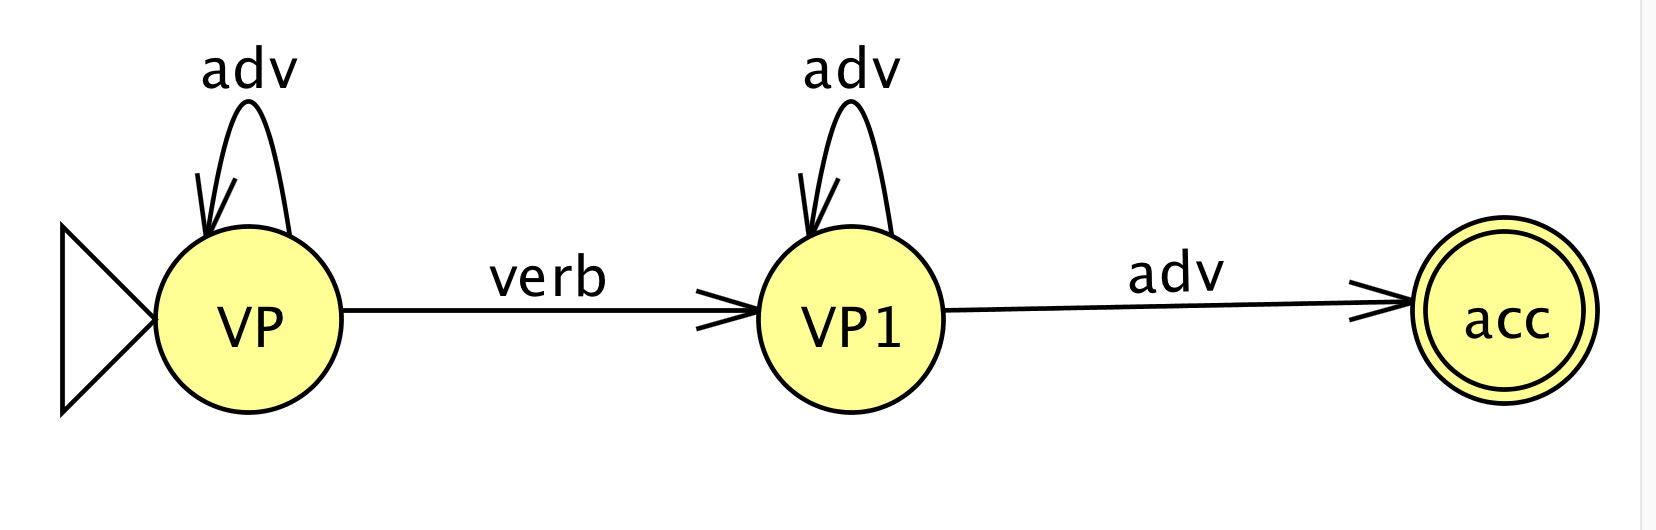
\includegraphics[width=.8\textwidth]{Grammar1.png}
\item Grammar \#2: \\ ~ \\
NP \ra art NP1 \\
NP \ra adj NP1 \\
NP1 \ra adj NP1 \\
NP1 \ra NP2 \\
NP2 \ra noun NP2 \\
NP2 \ra noun \\
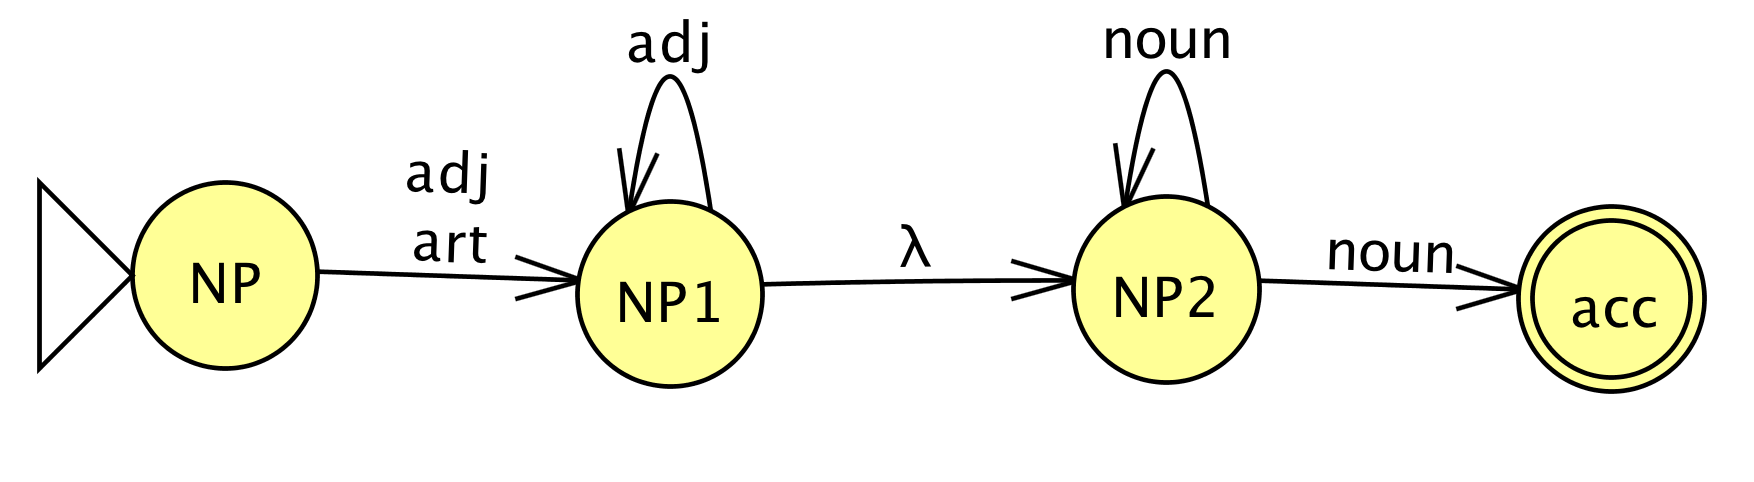
\includegraphics[width=.8\textwidth]{Grammar2.png}\newpage
\item Grammar \#3: \\ ~ \\
VP \ra VP1 \\
VP1 \ra VP2 \\
VP1 \ra VP3 \\
VP2 \ra aux VP3 \\
VP3 \ra verb \\
VP3 \ra verb adv\\
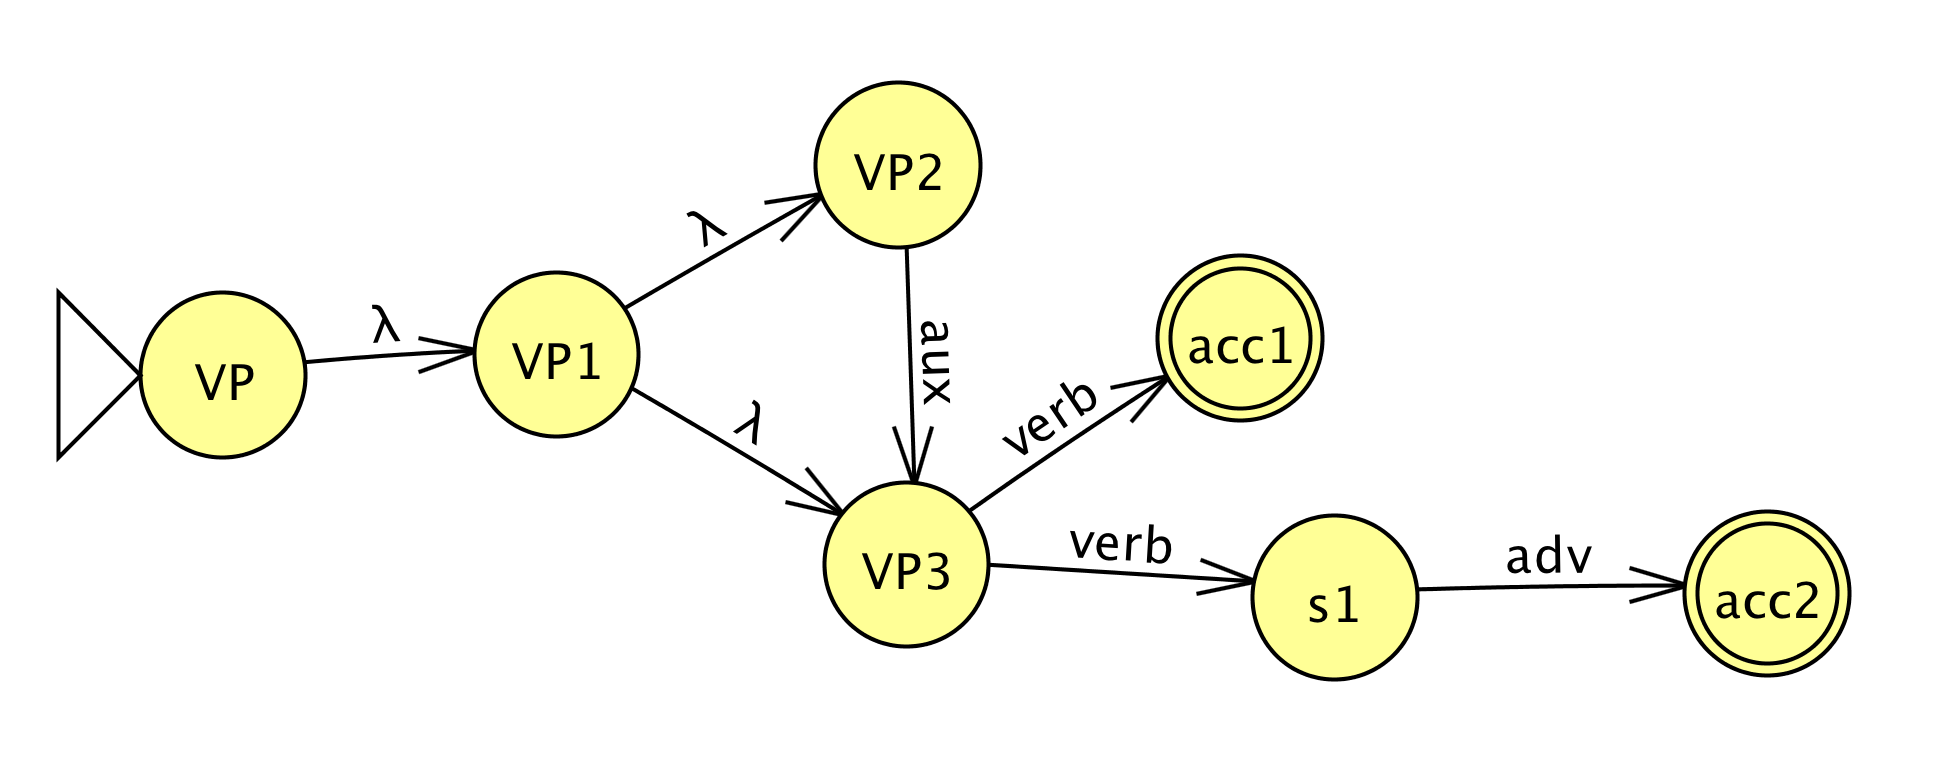
\includegraphics[width=.8\textwidth]{Grammar3.png}
\end{enumerate}


\newpage
\item (14 pts) Suppose your part-of-speech (POS) tagger assigned these
  POS tags to the sentence: 

\begin{quote}
the/{\sc art~}  light/{\sc noun~}  green/{\sc noun~} 
  candle/{\sc noun~}  shines/{\sc verb~}  green/{\sc adj~}
 light/{\sc noun~} \\  in/{\sc prep~}  the/{\sc art~} 
  green/{\sc adj~}  room/{\sc noun~}  to/{\sc prep~} 
  light/{\sc noun~}  the/{\sc art~}  room/{\sc noun~}
\end{quote}

Assume that the {\bf correct} POS tags for the sentence are:

\begin{quote}
the/{\sc art~}  light/{\sc adj~}  green/{\sc adj~} 
  candle/{\sc noun~}  shines/{\sc verb~}  green/{\sc adj~}
 light/{\sc noun~} \\  in/{\sc prep~}  the/{\sc art~} 
  green/{\sc adj~}  room/{\sc noun~}  to/{\sc inf~} 
  light/{\sc verb~}  the/{\sc art~}  room/{\sc noun~}
\end{quote}

Based on the information above, answer the questions
below. \underline{Leave your answers in fractional form!} 

\begin{enumerate}

\item What is the overall accuracy of your POS tagger?\\ ~ \\
11/15\\

\item What is the recall of your POS tagger for verbs?\\ ~ \\
1/2\\
\item What is the precision of your POS tagger for verbs? \\ ~ \\
1/1\\
\item What is the recall of your POS tagger for nouns?\\ ~ \\
4/4\\
\item What is the precision of your POS tagger for nouns?\\ ~ \\
4/7\\

\item What is the recall of your POS tagger for prepositions ({\sc prep})?\\ ~ \\
1/1\\
\item What is the precision of your POS tagger for prepositions ({\sc prep})?\\ ~ \\
1/2\\

\end{enumerate}




\newpage
\item (15 pts) Imagine that you have a collection of 1,200 documents
  and humans have labeled them with topics (e.g., politics, sports,
  etc.) Each document is assigned one topic.  Let's call this your
  ``annotated corpus''.  Suppose you have developed a machine learning
  (ML) classifier to automatically label a document with a topic, and
  you decide to evaluate its performance using cross-validation on the
  annotated corpus.

\begin{enumerate}

\item If you perform 3-fold cross-validation:
\begin{enumerate}
\item How many classifiers will you train? \\ ~ \\
Three classifiers will be trained.\\
\item How many documents will each of those classifiers be trained on?\\ ~ \\
Each classifier will be trained on 800 documents or 2/3 of the corpus.\\
\item How many documents will each of those classifiers be tested on?\\ ~ \\
Each classifier will be tested on the remaining 400 documents which were not used during training.\\
\end{enumerate}

\item If you perform 8-fold cross-validation:
\begin{enumerate}
\item How many classifiers will you train?\\ ~ \\
Eight classifiers will be trained.\\
\item How many documents will each of those classifiers be trained on? \\ ~ \\
Each classifier will be trained on 1050 documents, or 7/8 of the corpus.\\
\item How many documents will each of those classifiers be tested on?\\ ~ \\
Each classifier will be tested on the 150 documents not used for training.\\
\end{enumerate}

\item Suppose you have an extremely small amount of annotated data. 
  Would it be better to use a relatively small number of folds for
  cross-validation or a relatively large number of folds? Briefly explain your
  answer.\\ ~ \\ 
Using the numbers in the problem as an example, a larger fold count
(8) would be preferable to smaller fold count (3), assuming both
choices could be used to train classifiers with similar
accuracies. When using a larger fold count, in this scenario, we can
get a better sense of the variance of the mean test-accuracy due to
having more samples of model accuracies.  Considering the estimation
of how well the model generalizes is not appreciably better between
the two choices, since the probability of having a given accuracy on a
400 sample test is not appreciably better than getting the same
accuracy on a 150 sample test, especially as the number of labels
increases. Also, when using a larger fold fold count, we are more
likely to be training the models on a representative training set,
expecially when we have uncommon labels. Taken together it seems
preferable to use a classifier trained on many models that has been
tested ``more'' than than one trained of fewer models.

\end{enumerate}


\newpage
\underline{\textbf{Question \#6 is for CS-6340 students ONLY!}}  \\

\item (24 pts) Consider the grammar G below:

\begin{center}
\begin{tabular}{|ll|} \hline
\textbf{Grammar} & ~ \\  
S $\rightarrow$ NP VP    & NOUN \ra John \\
S $\rightarrow$ VP NP    & NOUN \ra can \\
NP $\rightarrow$ NOUN    & NOUN \ra well \\
VP $\rightarrow$ MOD VP1 & VERB \ra swim \\
VP1 $\rightarrow$ VERB   & MOD \ra can \\
VP1 $\rightarrow$ VERB ADV & ADV \ra well \\  \hline
\end{tabular}
\end{center}

List all of the entries that would be put on the chart by the Earley
parsing algorithm when parsing the sentence {\bf ``John can swim
  well''}.  Each chart entry should be a constituent or a rule, with a
start and end position indicating which words have been matched by the
constituent or rule. Assume that ``John'' is in position 1 and
``well'' is in position 4.

To get you started, the list below contains the chart entries for all
of the part-of-speech tag constituents. Your job is to complete
this list by adding the rest of the constituents and rules that would
be added to the chart during parsing.

For the rules, please use an asterisk (*) to separate the components
of the rule that have been matched from the ones that have not yet
been matched. For example, the rule: \\ {\bf ``S $\rightarrow$ * NP VP
  [1-1]''} means that nothing in this rule has been matched yet but
the rule can begin matching constituents starting in position 1.  The
rule {\bf ``S $\rightarrow$ NP * VP [1-2]''} means that the NP has
been matched in position 1-2 and the rule is waiting to match a VP
starting in position 2.

\begin{center}
{\bf CHART ENTRIES FOR ``John can swim well''} 

\begin{tabular}{lc} 
{\bf Constituent or Rule~~~} & {\bf ~~~Start-End} \\ \hline
NOUN(``John'') &  [1-2] \\
NOUN(``can'') & [2-3] \\
MOD(``can'') & [2-3] \\
VERB(``swim'') & [3-4] \\
NOUN(``well'') & [4-5] \\
ADV(``well'') & [4-5] \\
S $\rightarrow$ * VP NP & [1-1]\\
VP $\rightarrow$ * MOD VP1 & [1-1]\\
S $\rightarrow$ * NP VP & [1-1]\\
NP $\rightarrow$ * NOUN & [1-1]\\
NP $\rightarrow$ NOUN * & [1-2]\\
NP & [1-2]\\
%NOUN(``John'') &  [1-2] \\
S $\rightarrow$ NP * VP & [1-2] \\
VP $\rightarrow$ * MOD VP1 & [2-2] \\
VP $\rightarrow$ MOD * VP1 & [2-3] \\
%MOD(``can'') & [2-3] \\
VP1 $\rightarrow$ * VERB & [3-3] \\
VP1 $\rightarrow$ * VERB ADV & [3-3] \\
VP1 $\rightarrow$ VERB * & [3-4] \\
VP1 & [3-4]\\
%VERB(``swim'') & [3-4] \\
VP $\rightarrow$ MOD VP1 * & [2-4] \\
VP & [2-4] \\
S $\rightarrow$ NP VP * & [1-4] \\
S & [1-4] \\
VP1 $\rightarrow$ VERB * ADV & [3-4] \\
%VERB(``swim'') & [3-4] \\
VP1 $\rightarrow$ VERB ADV * & [3-5] \\
%ADV(``well'') & [4-5] \\
VP1 & [3-5] \\
VP $\rightarrow$ MOD VP1 * & [2-5] \\
VP & [2-5] \\
S $\rightarrow$ NP VP * & [1-5] \\
S & [1-5] \\
\end{tabular}
\end{center}



\end{enumerate}  % END OF WRITTEN QUESTIONS




\newpage
\hspace*{1.5in}  {\bf ELECTRONIC SUBMISSION INSTRUCTIONS} \\

You should submit your answers to the written assignment {\bf in pdf format}
on our course's CANVAS site by Friday, September 29 at 11:00pm.

\end{document}


